%\documentclass[11pt,aspectratio=169]{beamer}
\documentclass[11pt,aspectratio=169,handout]{beamer}

\usetheme{Boadilla}
\usepackage[utf8]{inputenc}
\usepackage[T1]{fontenc}
\usepackage{lmodern}
\usepackage{lipsum}
\usetheme{default}
\usepackage{cancel}
\usepackage{xcolor}

\usepackage{amsmath}
\usepackage{listings}
\lstset{language=[90]Fortran,
	basicstyle=\small\ttfamily,
	showtabs=false,
	tabsize=2,      
	keywordstyle=\color{red},
	commentstyle=\color{green},
	morecomment=[l]{!\ }% Comment only with space after !
}

%---- integration and diff ----------------------------------------------------
\newcommand{\ddif}[2][]{\mathrm{d}^{#1}#2}
\newcommand{\partdif}[2][]{\frac{\partial^{#1}}{\partial{#2}^{#1}}}
\newcommand{\dif}[3][]{\frac{\mathrm{d}^{#1}#3}{\mathrm{d}{#2}^{#1}}}
\newcommand{\integral}[4][]{\int_{#2}^{#3} \ddif[#1]{#4} \:}
\newcommand{\eval}[2]{\left. #1 \right\vert_{#2}}


\begin{document}
\author{Zejian Li \\(li.zejian@ictp.it)}
\title{Lecture 2-2: Differential Equations}
\subtitle{(Adapted from slides by Gerald Fux)}
%\logo{}
%\institute{}
\date{23. Oct. 2024}
%\subject{}
%\setbeamercovered{transparent}
%\setbeamertemplate{navigation symbols}{}


% ----------------------------------------------------------------
\begin{frame}[plain]
	\maketitle
\end{frame}


% ----------------------------------------------------------------

\begin{frame}
\frametitle{Introduction}
\begin{itemize}
	\item \textbf{Ordinary Differential Equations (ODE)}: 
	Differential equations for functions depending on only one variable.
	\pause
	\begin{itemize}
		\item Order of ODE: the highest appearing order of derivative of the function
		\pause
		\item System of ODE: coupled differential equation for multiple functions (each depending on only one variable).
	\end{itemize}
	\pause
	$$ \text{Bacteria growth} \quad \dif{t}{w} = \eta w \quad \text{is a 1st order ODE}$$
	\pause
	$$ \text{(Damped) harmonic oscillator} \quad \dif[2]{t}{x} = -\gamma \dif{t}x -\frac{k}{m} x \quad \text{is a 2nd order ODE}$$
	\pause
	\item \textbf{Partial Differential Equations (PDE)}:
	Differential equations for functions depending on multiple variables.
	For example: Maxwell differential equations are a system of first order PDE.
\end{itemize}
\pause
We want to find the unknown function(s) [e.g. $w(t)$, $x(t)$, or $\vec{E}(\vec{r},t)$ \& $\vec{B}(\vec{r},t)$] for specific initial conditions.
\end{frame}


\begin{frame}
\frametitle{Numerical Methods for Differential Equation}
\begin{itemize}
	\item Often analytical solutions are complicated, hard to find, or unknown.
	\pause
	\item Even more often there exist no analytical solutions, and a numerical solution is necessary.
	\pause
	\item Numerical method idea:
	\begin{itemize}
		\item Start with the initial conditions.
		\pause
		\item Take a small step: Calculate an approximate value of the function for a small increment of the independent variable.
		\pause
		\item Take another small step: Calculate the next approximate value of the function for another small increment of the independent variable.
		\item $\ldots$ and so on $\ldots$
	\end{itemize}
\end{itemize}
\end{frame}


\begin{frame}
\frametitle{Euler Method - Idea}
For 1st order ODE, which have the form:
$$ \dif{t}{x} = f(t, x) \quad \text{with} \quad x(t_0) = x_0 $$
\pause
For example:
$$ \text{radioactive decay:} \quad \dif{t}{x} = f(\cancel{t},x) = -\gamma x$$ 
\pause
Consider the Taylor expansion at $t=t_0$ of the solution $x(t)$:
$$ x(t_0+\Delta t) = x(t_0) + \Delta t \cdot \eval{\dif{t}{x}}{t=t_0} + \mathcal{O}(\Delta t^2)$$
\vspace*{-3ex}
\pause
\begin{block}{\vspace*{-3ex}}
	$$ \quad x(t_0+\Delta t) \quad \approx \quad x(t_0) + f(t_0, x_0) \cdot \Delta t$$
\end{block}
\end{frame}


\begin{frame}
\frametitle{Euler Method - Sketch}
\begin{block}{\vspace*{-3ex}}
	$$ \quad x(t_0+\Delta t) \quad \approx \quad x(t_0) + f(t_0, x_0) \cdot \Delta t$$
\end{block}
\begin{figure}
	\centering
	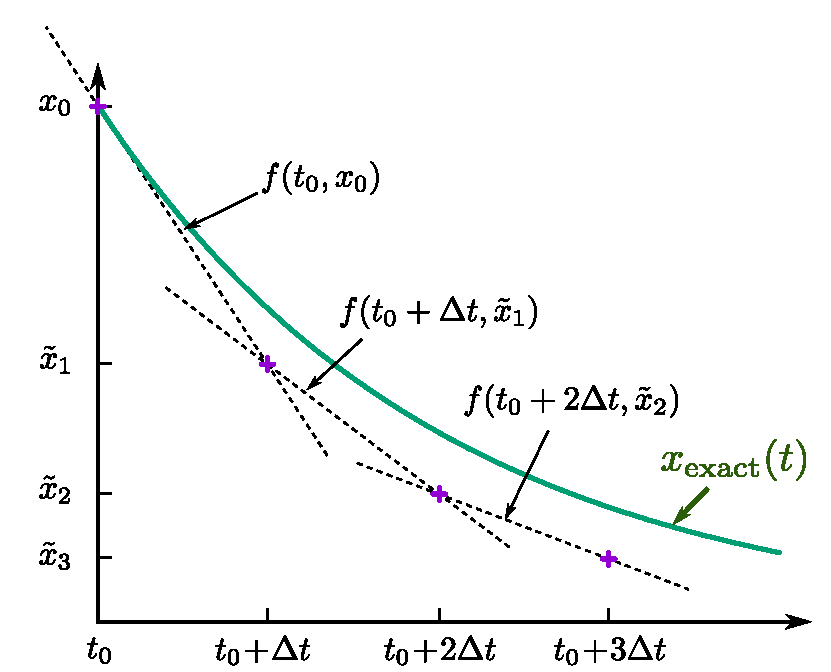
\includegraphics[width=0.5\textwidth]{fig/diffeq-euler}
\end{figure}%
\end{frame}


\begin{frame}
\frametitle{Euler Method - Algorithm}
\begin{columns}
\column{0.4\textwidth}
\begin{figure}
	\centering
	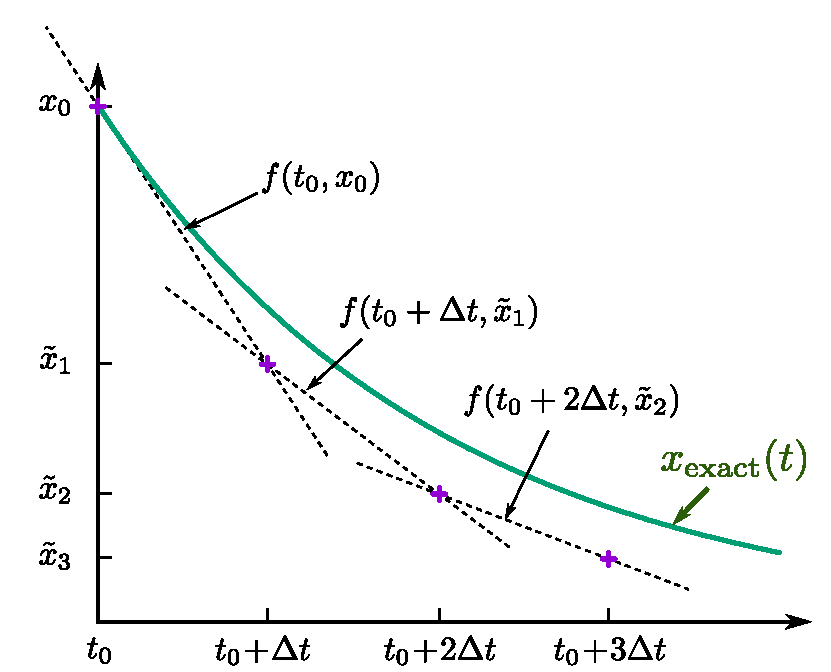
\includegraphics[width=0.9\textwidth]{fig/diffeq-euler}
\end{figure}%
\column{0.55\textwidth}
\begin{block}{Algorithm: Euler Method}
	\pause
	\textbf{Input}: function $f(t,x)$, initial values $t_0$, $x_0$, step size $\Delta t$, and number of steps $N$
	\pause
	\begin{enumerate}
		\item set $x := x_0$ and $t := t_0$
		\pause
		\item repeat $N$ times:
		\pause
		\begin{itemize}
			\item set $fx := f(t, x)$
			\pause
			\item set $x := x + fx \cdot \Delta t$
			\pause
			\item set $t := t + \Delta t$
		\end{itemize}		
	\end{enumerate}  
	\pause
	\textbf{Output}: the sequence of $t$ and $x$ approximating the solution of $\dif{t}{x} = f(t,x)$.
\end{block}
\end{columns}
\end{frame}

\begin{frame}[fragile]
\label{slide:euler-code}
\frametitle{Euler Method - Fortran Implementation Sketch}
\begin{lstlisting}	
subroutine euler_method(t0, x0, dt, N, tlist, xlist)
	! ... variable declarations and allocations ...
	x = x0
	t = t0
	tlist(1) = t
	xlist(1) = x         
	do i = 1, N
		fx = f(t,x)
		x = x + fx * dt
		t = t + dt
		tlist(i+1) = t
		xlist(i+1) = x
	end do
end subroutine euler_method

\end{lstlisting}
\end{frame}

\begin{frame}
\frametitle{Improved Euler Method: Midpoint Method}
In a similar spirit to the improvement from the left Riemann sum to the midpoint sum for numerical integration, one can also improve the Euler method for differential equations:

$$x(t_0 + \Delta t) \approx x(t_0) + \Delta t \cdot \eval{\dif{t}{x}}{{\color{red}t=t_M}} + \mathcal{O}(\Delta t^{\color{red}3}) \quad \text{with} \quad {\color{red}t_M=t_0 + \Delta t/2}$$

\pause

\begin{block}{\vspace*{-3ex}}
\begin{align*}
x(t_0+\Delta t) \quad &\approx \quad x(t_0) + f(t_M, x_M) \cdot \Delta t \\
 & \text{with} \\
t_M \quad &:= \quad t_0+\Delta t/2 \\
x_M \quad &:= \quad x(t_0) +  f(t_0, x_0)\cdot \Delta t/2
\end{align*}
\end{block}
\end{frame}

\begin{frame}
\frametitle{Higher Order ODE $\rightarrow$ System of 1st Order ODE}
Euler method and midpoint method only work for 1st order ODEs. However, $\ldots$
\pause
\begin{block}{\vspace*{-3ex}}
	It is always possible to rewrite a higher order ODE as a system of 1st order ODEs!
\end{block}
\pause
For example, the equation of motion for the angle $x$ of a friction-less (stiff) pendulum
$$\dif[2]{t}{x} = -\sin(x)$$
can be rewritten as the system of two first order ODEs (for the angle $x$ and the angular velocity $v$):
\begin{align*}
	\dif{t}{x} &= v \\
	\dif{t}{v} &= -sin(x) \mathrm{.}
\end{align*} 
\end{frame}

\begin{frame}
\frametitle{Euler Method - Algorithm for a System}
\label{slide:euler-system}
\begin{block}{Algorithm: Euler Method for a System $x$ and $y$}
	\textbf{Input}: functions $f_x(t,x,y)$, $f_y(t,x,y)$, initial values $t_0$, $x_0$, $y_0$, step size $\Delta t$, and number of steps $N$
	\pause
	\begin{enumerate}
		\item set $x := x_0$, $y := y_0$ and $t := t_0$
		\item repeat $N$ times:
		\pause
		\begin{itemize}
			\item set $fx := f_x(t, x, y)$
			\item set $fy := f_y(t, x, y)$
			\pause
			\item set $x := x + fx \cdot \Delta t$
			\item set $y := y + fy \cdot \Delta t$
			\pause
			\item set $t := t + \Delta t$
		\end{itemize}		
	\end{enumerate}  
	\textbf{Output}: the sequence of $t$, $x$, and $y$ which approximates the solution of 
	\begin{align*}
		\dif{t}{x} &= f_x(t,x,y) & 
		\dif{t}{y} &= f_y(t,x,y).
	\end{align*}
\end{block}
\end{frame}

\begin{frame}{Assignment 12}
	Write a program that solves the differential equation $\frac{\mathrm{d} x}{\mathrm{d} t} = -x$ using 1) Euler and 2) midpoint methods.\pause
	\begin{itemize}
		\item Create separate subroutines for the two methods (see slide 7).\pause
		\item Solve with initial conditions \texttt{x(0.0) = 1.0} and \texttt{dt=0.1, N=100} and store the results in arrays \texttt{tlist} and \texttt{xlist}.\pause
		\item The program should create a file for each method (\texttt{euler.txt} and \texttt{midpoint.txt}) with the result in two columns: \texttt{t} and \texttt{x(t)}.\pause
		\item Plot the result $x$ versus $t$ with your favorite plotting program.\pause
		 
	\end{itemize}
\textbf{Bonus question:}
		\begin{itemize}
			\item Expand your subroutines and solve the equation of motion for the angle $x$ of a friction-less physical pendulum: $\frac{\mathrm{d}^2 x}{\mathrm{d} t^2} = -\sin(x)$ using the two methods, with initial conditions \texttt{t0=0, x0=1.0, v0=0.0} and \texttt{dt = 0.1, N=300}.
		\end{itemize}
		Submit the graphs and your code as \texttt{Ass12.YourLastName.f90} to \texttt{li.zejian@ictp.it} before the next lesson.
\end{frame}


\begin{frame}
\frametitle{Reminder for plotting:}
\begin{itemize}
	\pause
	\item You can use whatever program you like to plot the dynamics. A very simple way is to use \texttt{gnuplot}.
	\begin{itemize}
		\pause
		\item If the file 'data.txt' has two columns $t$ and $x$, then you can plot $x(t)$ with:\\
		\texttt{\$ gnuplot -p -e "plot 'data.txt' using 1:2 with lines"}
		\pause
		\item If the file 'data.txt' has three columns $t$, $x$, and $v$, then you can plot $x(t)$ and $v(t)$ with:\\
		\texttt{\$ gnuplot -p -e "plot for [col=2:3] 'data.txt' using 1:col with lines"}
	\end{itemize} \pause
	\textbf{Side note:}
	\begin{itemize}
		\item Usually we need a much smaller \texttt{dt} to obtain reliable results. Here we use the relatively large \texttt{dt=0.1} to better compare the performance of the difference methods.
	\end{itemize}
\end{itemize}

\end{frame}

\end{document}